\section{Related Work}

There is clearly demand for a multidimensional alternative to the fitness landscape metaphor which can help develop the intuition for evolutionary space provided by such a simple visualization. Multiple approaches to this multidimensional problem currently exist; however, they suffer from problems with scaling  and in some cases fail to provide intuition about the movement of lineages across the space over evolutionary time.

Here we present the current standard in fitness landscape visualization in more than two dimensions, as well as inspirations for our own extension into 3D and 4D landscape-based visualizations in virtual reality. 

\subsection{Graph-Based Visualizations}

The current standard for visualizations beyond two dimensions is to present a graph-based model. 
The most typical representation, which we term network models, is to represent the search space as sparsely connected network.
An alternative model termed Hyper-Space Graph Paper instead represents the space as a grid of systematically arranged trait combinations.

\subsubsection{Network Models}

\begin{figure}
    \centering
    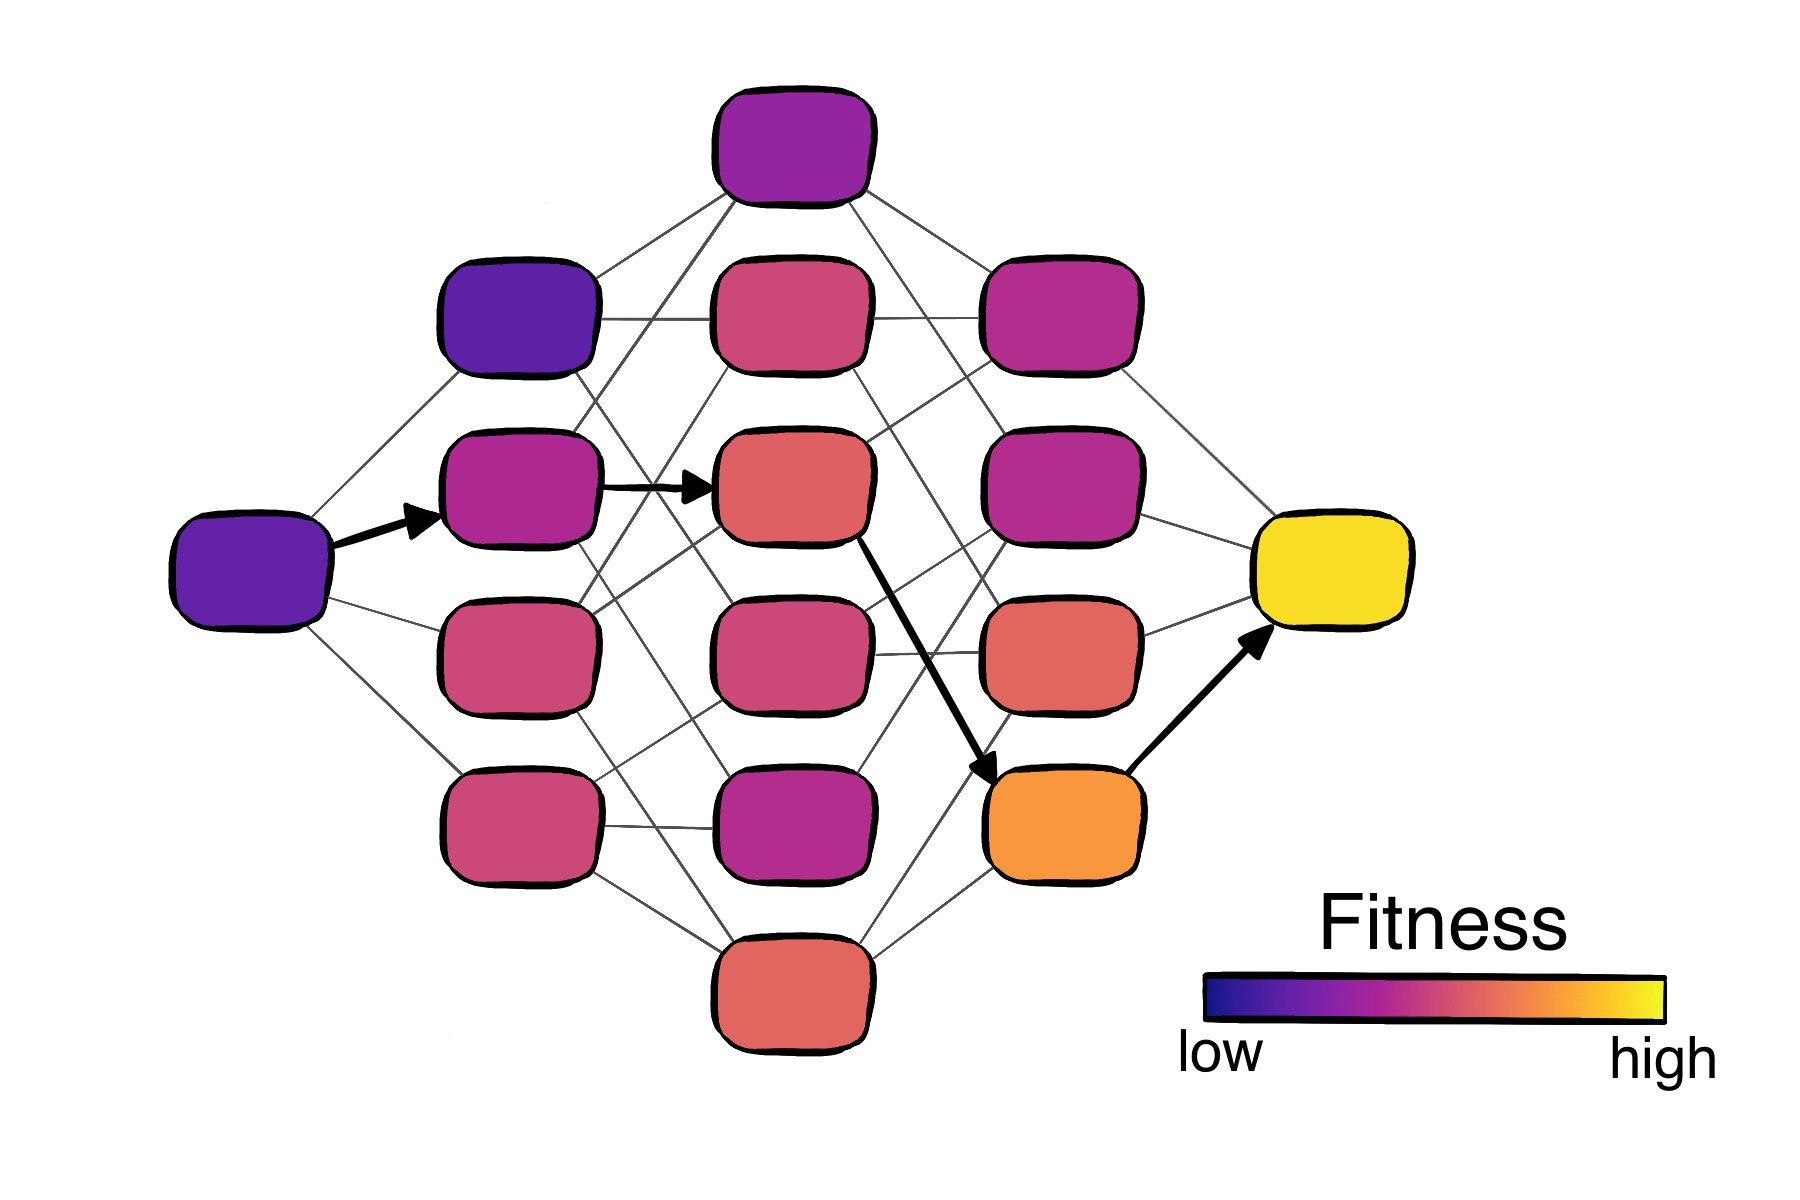
\includegraphics[width=0.5\textwidth]{chapters/3-vr-viz/figs/network.png}
    \caption{Network model of a fitness landscape. Lines indicate genotypes which are adjacent in evolutionary space. Colors indicate fitness according to key. Arrows denote traversal of the landscape. Adapted from Wu et al., 2016. Image by Katie Gleason.}
    \label{fig:related-work:network}
\end{figure}

Network models are perhaps the most popular way to represent higher dimensional evolutionary search spaces.
In these models, nodes represent genotypes while edges represent proximity; connected nodes are adjacent genotypes. \citep{mccandlish_visualizing_2011}.
Directed edges in these visualizations can represent either the observed behavior of a lineage traversing the space, or the direction of increasing fitness.
Lineage trajectories are also sometimes represented by the color of edges and node outlines \citep{ogbunugafor_competition_2017}.
Fitness can be represented visually in a multitude of ways: as labels on the nodes \citep{ogbunugafor_competition_2017}, node size \citep{mccandlish_visualizing_2011, iram_controlling_2021}, or colorings of the network \citep{wu_adaptation_2016, jimenez_comprehensive_2013}. 
An example of a network model with fitness mapped to node colorings is provided in \autoref{fig:related-work:network}.

A common use of network models is to represent landscapes composed of presence/absence data for a small number of genes (often four). In evolutionary medicine, a number of empirically-derived landscapes of this form exist \citep{mira_rational_2015, ogbunugafor_adaptive_2016}. With four genes to consider, there are 16 possible genotypes. These 16 genotypes can be arranged in an intuitive pattern where all mutationally-adjacent genotypes are adjacent to each other. Such a landscape is four dimensional (indeed, these visualizations are sometimes referred to as tesseracts). However, this intuitive visual representation is only possible because each of the dimensions is constrained to the values zero and one. %Intuitive graph layouts are more challenging for five dimensions, and have yet to be discovered for higher number of dimensions.

Overall, network models do not suffer the information loss problem of 2D and 3D topological representations; every candidate genotype is represented as a node in the network. 
Proximity in evolutionary space is also intuitive, represented by edges connecting nodes. 
However, intuition is limited by the size of the network, which is determined by the number of traits as well as the number of values each trait can take on.
For very large networks, visualization quickly becomes messy as the number of edges grows rapidly.  
Additionally, dynamics of interest such as ruggedness valley crossing are difficult to visualize; however, see \citep{ogbunugafor_competition_2017} for one visual option.
Finally, a particularly difficult limit of network models is that they are by necessity discrete; continuous-valued landscapes or lineages cannot be visualized with a finite number of nodes.

\subsubsection{Hypergraphs}

Hyperspace Graph Paper (HSGP) is an alternative graph-based model that takes advantage of recursive structure to aid in intuition. 
HSGP represents binary strings of length $n$ as the corners of an $n$-dimensional hypercube, then ``unfolds" that cube to produce a flat grid representation \citep{wiles_hyperspace_2006}. 
Adjacent genotypes have self-similar placement within sub-grids, and fitness is represented via shading (\autoref{fig:related-work:hgsp}). 

\begin{figure}
    \centering
    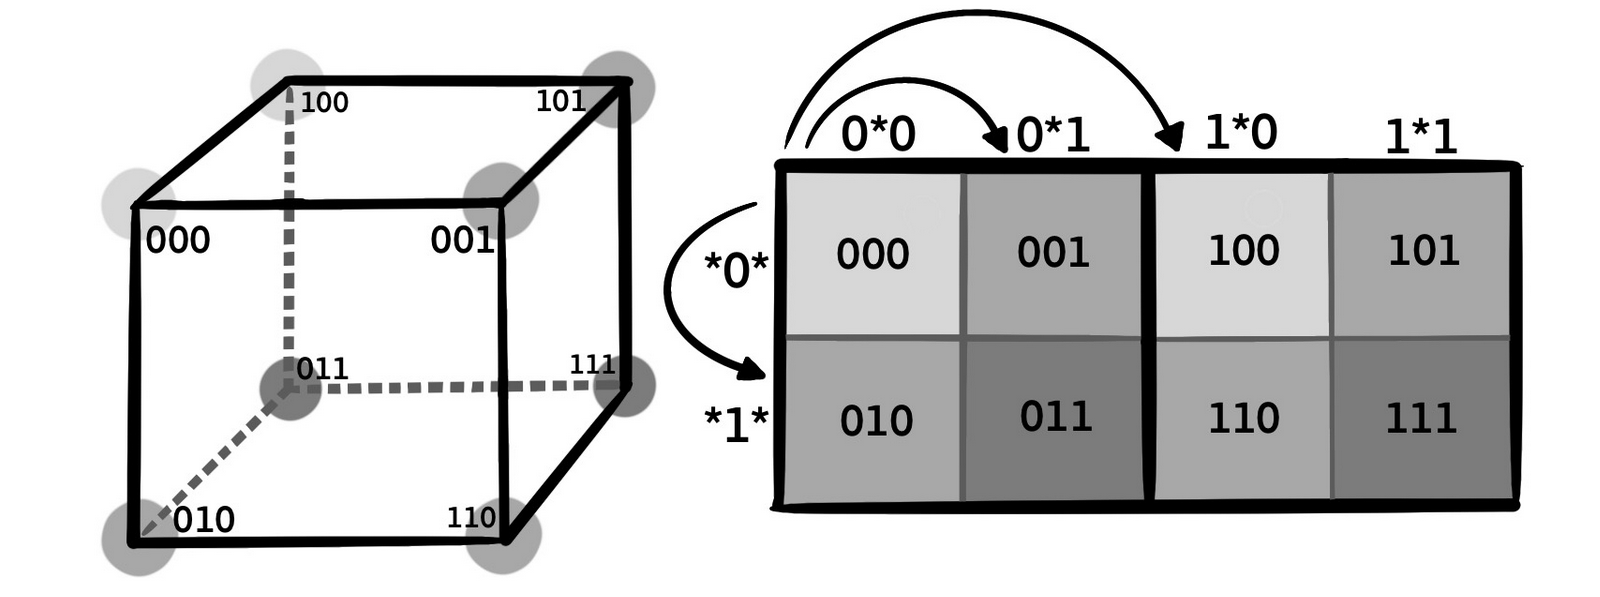
\includegraphics[width=0.5\textwidth]{chapters/3-vr-viz/figs/hsgp.png}
    \caption{Hyperspace graph paper example in 3D. Each corner of the cube is ``unfolded" to create a flat grid structure. Arrows are for demonstration purposes to indicate how adjacent corners in the cube are positioned in the unfolded grid. Greyscale represents fitness, where more saturated greys are higher fitness. Adapted from Wiles et al., 2003. Image by Katie Gleason.}
    \label{fig:related-work:hgsp}
\end{figure}

One advantage of HSGP visualizations, as in the network models, is that they are lossless; each point in fitness space directly translates to a position in the grid, so no information is discarded. 
Unlike network models, edges are not explicitly drawn, reducing the visual noise for larger landscapes. 
For HSGP models it is possible to view global and local maxima at a glance, even in problems with multiple optima \citep{wiles_mapping_2003}. 
However, they still share one of the major shortcomings of network models: they are limited to discrete landscapes, and in particular to landscapes which can be binary-coded. 
Additionally, since adjacency in evolutionary space does not map directly to adjacency in the visualization, viewing lineage traversals across the landscape is messy and unintuitive. 

Network-based models do not suffer from the same dimensionality loss as landscape-based models, but this ability to expand to multiple dimensions does not necessarily mean those expansions are intuitive.
Many of the limitations of network-based models are due to either attempting to combine a lot of information into limited spatial dimensions (i.e.~a 2D image) or due to their lack of spatial structure (i.e.~poor representation of proximity in genotype space vs.~fitness space). 
Therefore, we turn to more spatially-based models to build intuition for higher dimensions.

\subsection{VR-Enabled Visualizations}

Virtual reality is increasingly used to push the boundaries of data visualization. Previous studies have shown the use of VR can support better intuition for spatial data \citep{ambinder_human_2009}, provide a faster overview for big data visualizations \citep{olshannikova_visualizing_2015}, and provide deeper insight into the true structure of imaging-related data \citep{el_beheiry_virtual_2019}. However, the use of VR to study evolutionary data generally, and fitness landscapes specifically, has been extremely limited.

\subsubsection{2D Landscapes in VR}

\begin{figure}
    \centering
    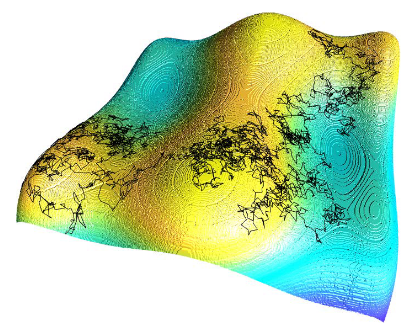
\includegraphics[width=0.5\textwidth]{chapters/3-vr-viz/figs/2dviz.png}
    \caption{2D landscape visualized in virtual reality. Black line represents a lineage traversing the landscape.}
    \label{fig:related-work:2dviz}
\end{figure}

There is no prior work on using VR to visualize higher-dimensional landscapes, but VR has been used to visualize 2D fitness landscapes \citep{dolson_visualizing_2018, dolson_interpreting_2020}. 
Here, as in the topological representation, the genotype is represented as a point on the cartesian plane. 
The spatial capabilities of VR are leveraged to show fitness as height, analogous to a 3D relief map (\autoref{fig:related-work:2dviz}. 
This use of VR avoids the problems inherent to projecting 3D graphs onto 2D pages or planes. 

The ability to visualize landscapes in their full spatial context allows for greater insight into evolutionary dynamics across the landscape; for example, lineages can be traced ``through" peaks rather than ``over" them \citep{dolson_visualizing_2018}. 
However, this visualization is still limited to 2D landscapes and therefore is subject to many of the same issues as the topographical projection, albeit with improved interpretibility and visibility. 

\subsubsection{Breaking into the Fourth Dimension}

It is relatively simple to imagine how one might represent a 3-dimensional landscape in a 3-dimensional space, but it is more difficult to imagine representations for a 4-dimensional landscape. 
The fourth dimension essentially must be projected into the 3-dimensional space, casting a 3-dimensional ``shadow". 
The viewer can then see slices of the fourth dimension by viewing 3D space. 
However, these slices cannot be viewed concurrently, so we require a way to step through successive slices. 

One option is to display 3D slices in a grid format, as in one medical application termed ``Bento Box" \citep{johnson_bento_2019}. 
This approach allows users to simultaneously view multiple slices, which can be helpful for comparative analysis. 
However, since this approach requires rendering all slices to the screen at once, it is computationally costly for the graphical software.

Another approach is to allow the viewer to scroll through three-dimensional slices, analogous to an MRI scan. 
Slices of a fourth-dimensional object are displayed one at a time, with the viewer able to scroll through the slices at will.
This allows for smoother rendering and user control, while sacrificing the comprehensive view from the Bento Box approach. 

Using a combination of inspiration from 2D fitness landscapes in VR and existing techniques to visualize 4D landscapes, we can identify key components to visualize 3- and 4-Dimensional fitness landscapes in virtual reality. 